\documentclass[10pt,a4paper]{article}
\usepackage[T1]{fontenc}\usepackage[utf8]{inputenc}\usepackage{geometry}\geometry{margin=2cm}
\usepackage{hyperref}\usepackage{tikz}\usetikzlibrary{positioning,arrows.meta}
\title{\texttt{hymeko\_graph}: CellTopology}\author{graph}\date{Created-at: 2026-09-24 00:25 CEST}
\begin{document}\maketitle
\section{Scope and justification}
Core-listed crate \texttt{hymeko\_graph}; additive change on branch \texttt{feat/cell-topology},
authorised by the user 2026-09-24. Justification: Nagare feature request
\texttt{reports/2026-09-24-feature-request-hymeko-graph-cell-topology.md} (about a dozen consumer types
re-declare signed uniform-arity incidence; \texttt{SignedHyperIncidence} has one scale, scalar
fields only, and no rank). \textbf{ETA $\approx$1.5 h}: module $\approx$45 min, tests and delegation
$\approx$30 min, gates and Nagare build against the branch $\approx$15 min.
\section{Interface (new, public)}
\texttt{cell\_topology::\{CellTopology, CellRank, CellTopologyError, ScalePolicy, RankScales,
RankIncidence, RankCofaces\}}. Width-$d$ \texttt{lower\_to\_cell}, \texttt{cell\_to\_lower}, their
adjoints and sign gradients on \texttt{RankIncidence}. \texttt{SignedHyperIncidence} keeps its API and
delegates its two contractions ($d=1$) to the one kernel owner.
\section{Numerical contract and tests}
(1) \texttt{SignedHyperIncidence} outputs bitwise equal to recordings made before the change;
(2) width-$d$ column $j$ equals the $d=1$ contraction of column $j$, bitwise;
(3) adjoint identities $\langle Ax,g\rangle=\langle x,A^\top g\rangle$ per direction;
(4) sign gradients match central differences; (5) cofaces equal a counting-sort reference and are
sorted with duplicates kept; (6) degrees and scale policies match their closed forms; (7) typed
refusals for zero arity, ragged/sign mismatch, member out of range. Then Nagare builds and passes
its suite with the dependency patched to this branch (command-line patch, no manifest edit).
\section{Budget, risk, rollback}
Toy fixtures; RSS $\ll$1 GB. Risk: re-associating an accumulation breaks bit parity --- guarded by (1)
and (2). No dependency change. Rollback: delete the branch.
\begin{figure}[h]\centering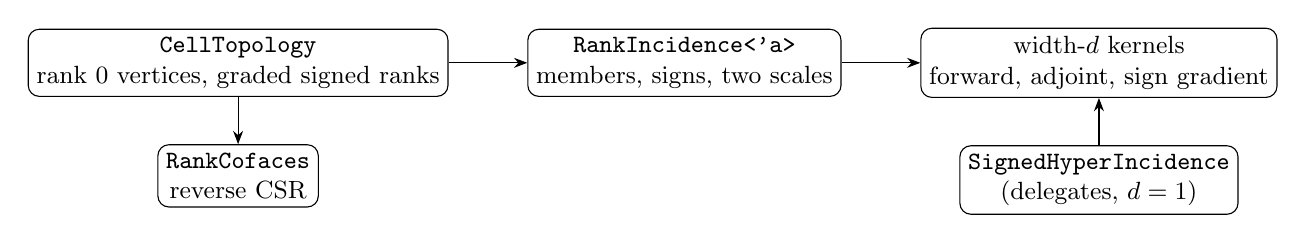
\begin{tikzpicture}[node distance=6mm and 10mm, box/.style={draw, rounded corners, align=center, font=\small, inner sep=3pt}, >=Stealth]
  \node[box] (topo) {\texttt{CellTopology}\\rank 0 vertices, graded signed ranks};
  \node[box, right=of topo] (view) {\texttt{RankIncidence<'a>}\\members, signs, two scales};
  \node[box, right=of view] (kern) {width-$d$ kernels\\forward, adjoint, sign gradient};
  \node[box, below=of topo] (csr) {\texttt{RankCofaces}\\reverse CSR};
  \node[box, below=of kern] (shi) {\texttt{SignedHyperIncidence}\\(delegates, $d=1$)};
  \draw[->] (topo) -- (view); \draw[->] (view) -- (kern); \draw[->] (topo) -- (csr); \draw[->] (shi) -- (kern);
\end{tikzpicture}
\end{figure}
\end{document}
